\documentclass[12pt]{article}

\usepackage{amsmath}
\usepackage{amssymb}
\usepackage{amsfonts}
\usepackage[style=iso]{datetime2}
\usepackage[explicit]{titlesec}
\usepackage{amsthm}
\usepackage{array}
\usepackage{graphicx}
\usepackage{float}
\usepackage{siunitx}

\graphicspath{ {./Images/} }

\theoremstyle{definition}
\newtheorem{problem}{Problem}
\newtheorem{definition}{Definition}

\begin{titlepage}
\title{Calculus I: Tangent Lines and Rates of Change}
\author{The Melon Man}
\date{\today}
\end{titlepage}

\renewcommand{\thesection}{\Roman{section}}

\allowdisplaybreaks

\setlength{\parindent}{0pt}
\setlength{\parskip}{1em}

\begin{document}
\maketitle

\section{Introduction}
Both tangents and rates of change are rather important to calculus.
They relate to the topic of limits which are a significant part of Calculus I as their own topic; limits are also used to provide some formal definitions for the other key parts of calculus.
By understanding these problems, we can look at limits, what they are and how they can be used to analyse the behaviour of functions.
Also, the rate of change problem that will be covered is incredibly important to limits and Calculus I as a whole.

\section{Tangent Lines}
Before we look at problems involving tangent lines, it would be best to define what they are.
For some point $x=a$ on a curve described by a function $f(x)$, a tangent line at that point is one that just touches the curve at that point.
In a certain way, we could consider the tangent to be 'parallel' to the curve.
Below is an example of a tangent line to some point.

\begin{figure}[H]
    \centering
    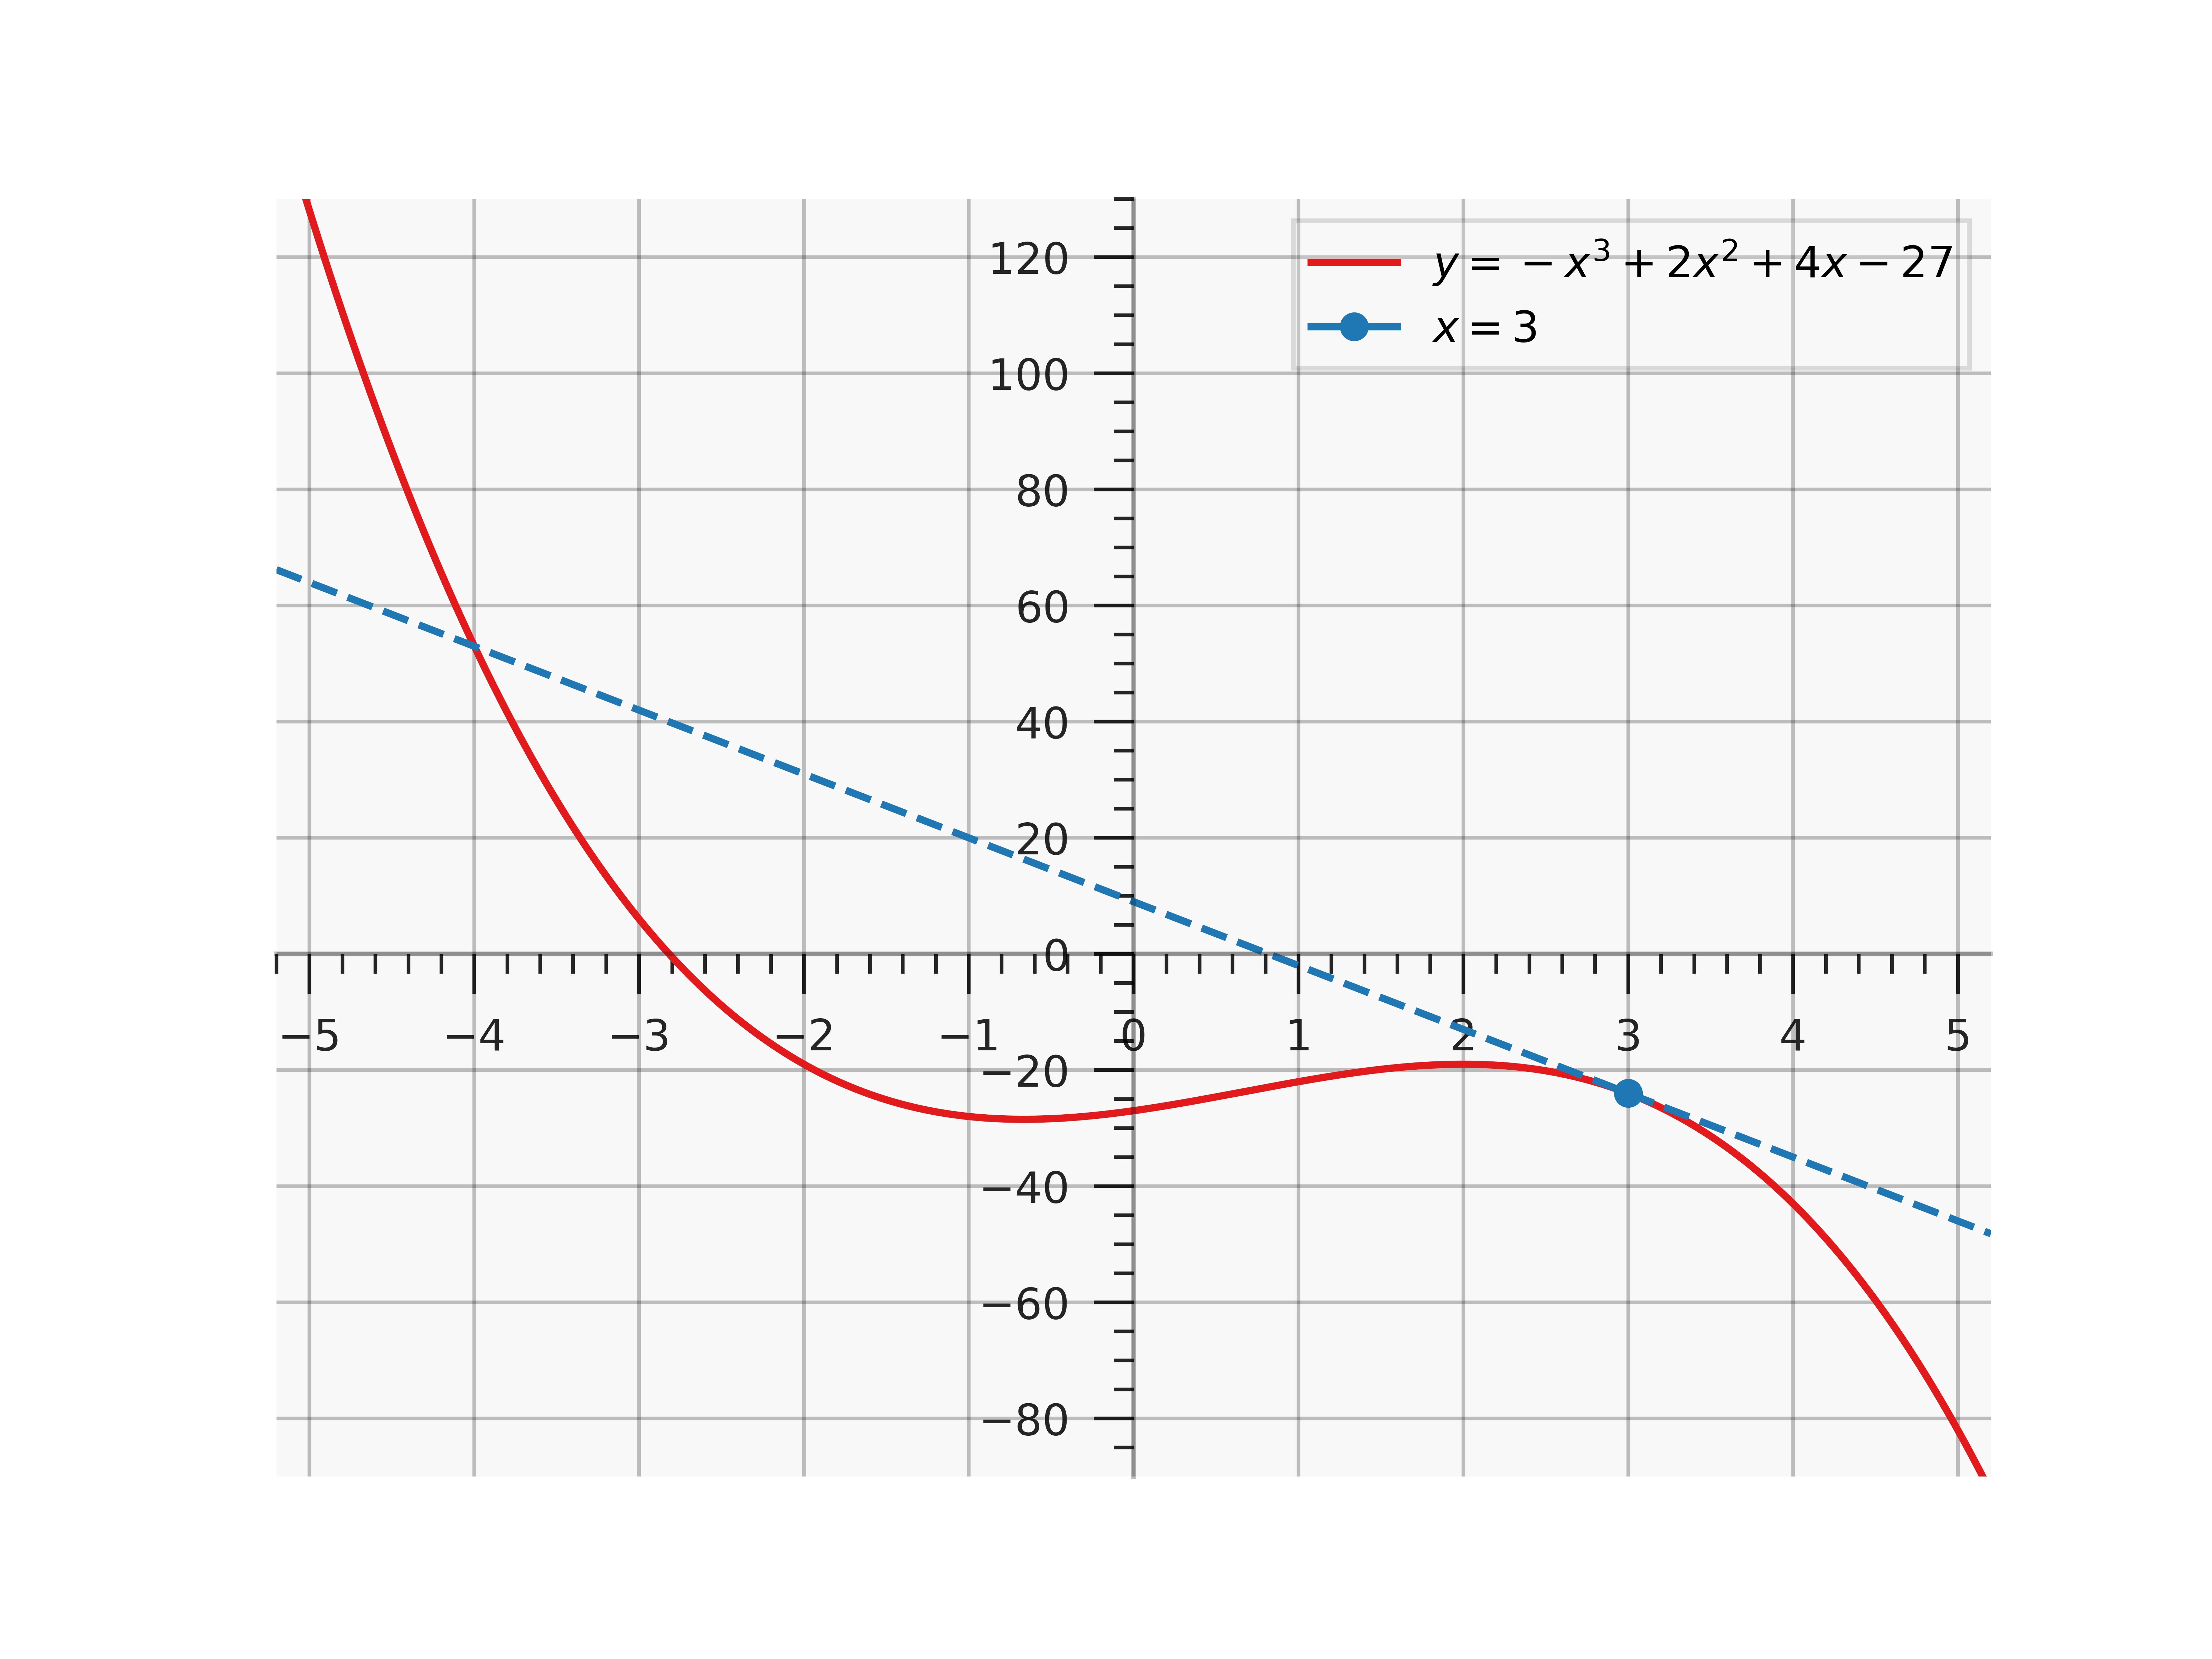
\includegraphics[width=12.5cm, keepaspectratio]{tangent_lines_1.png}
    \caption{Tangent Lines}
    \label{fig:fig1}
\end{figure}

Here, the straight blue line is tangent to the curve at $x=3$.
At that point, it touches the curve but just.
The line is going the same direction as the curve at that point; we could describe them as 'parallel'.
Notice that the line also touches the curve at $x=-4$, but does not appear 'parallel' to the curve at that point so we would not say that it is tangent to that point of the curve.
Instead, we may call it a secant line at that point as it intersects the curve at least twice.
With a definition of a tangent line, we can solve problems involving them.

\begin{problem}
Find the line tangent to $f(x)=-2x^2+15$ at $x=1$. \label{eq:1}
\end{problem}

To find the equation of the line, we either need two points on the line or one point and the slope.
We know that a line tangent to the curve at $x=1$ will touch the curve at that point.
Therefore, the point $(1, f(1))$ or $(1, 13)$ is a point on the line.
At this point, we do not have any more information about the tangent line.
We need another point on the line or its slope.
The slope is the important part as we would use that other point just to calculate the slope of the line.

To get the slope of the tangent line, we can start off with estimates.
First, let $P$ be the one point on the line we know: $P=(1,13)$.
We can define another point $Q$ such that it is a point on our curve: $Q=(x, f(x))$.
Let's take $x=2$ as an example.
We would have $Q=(2,7)$.
Below is the graph of the curve, our tangent line, and the secant line connecting $P$ and $Q$.

\begin{figure}[H]
    \centering
    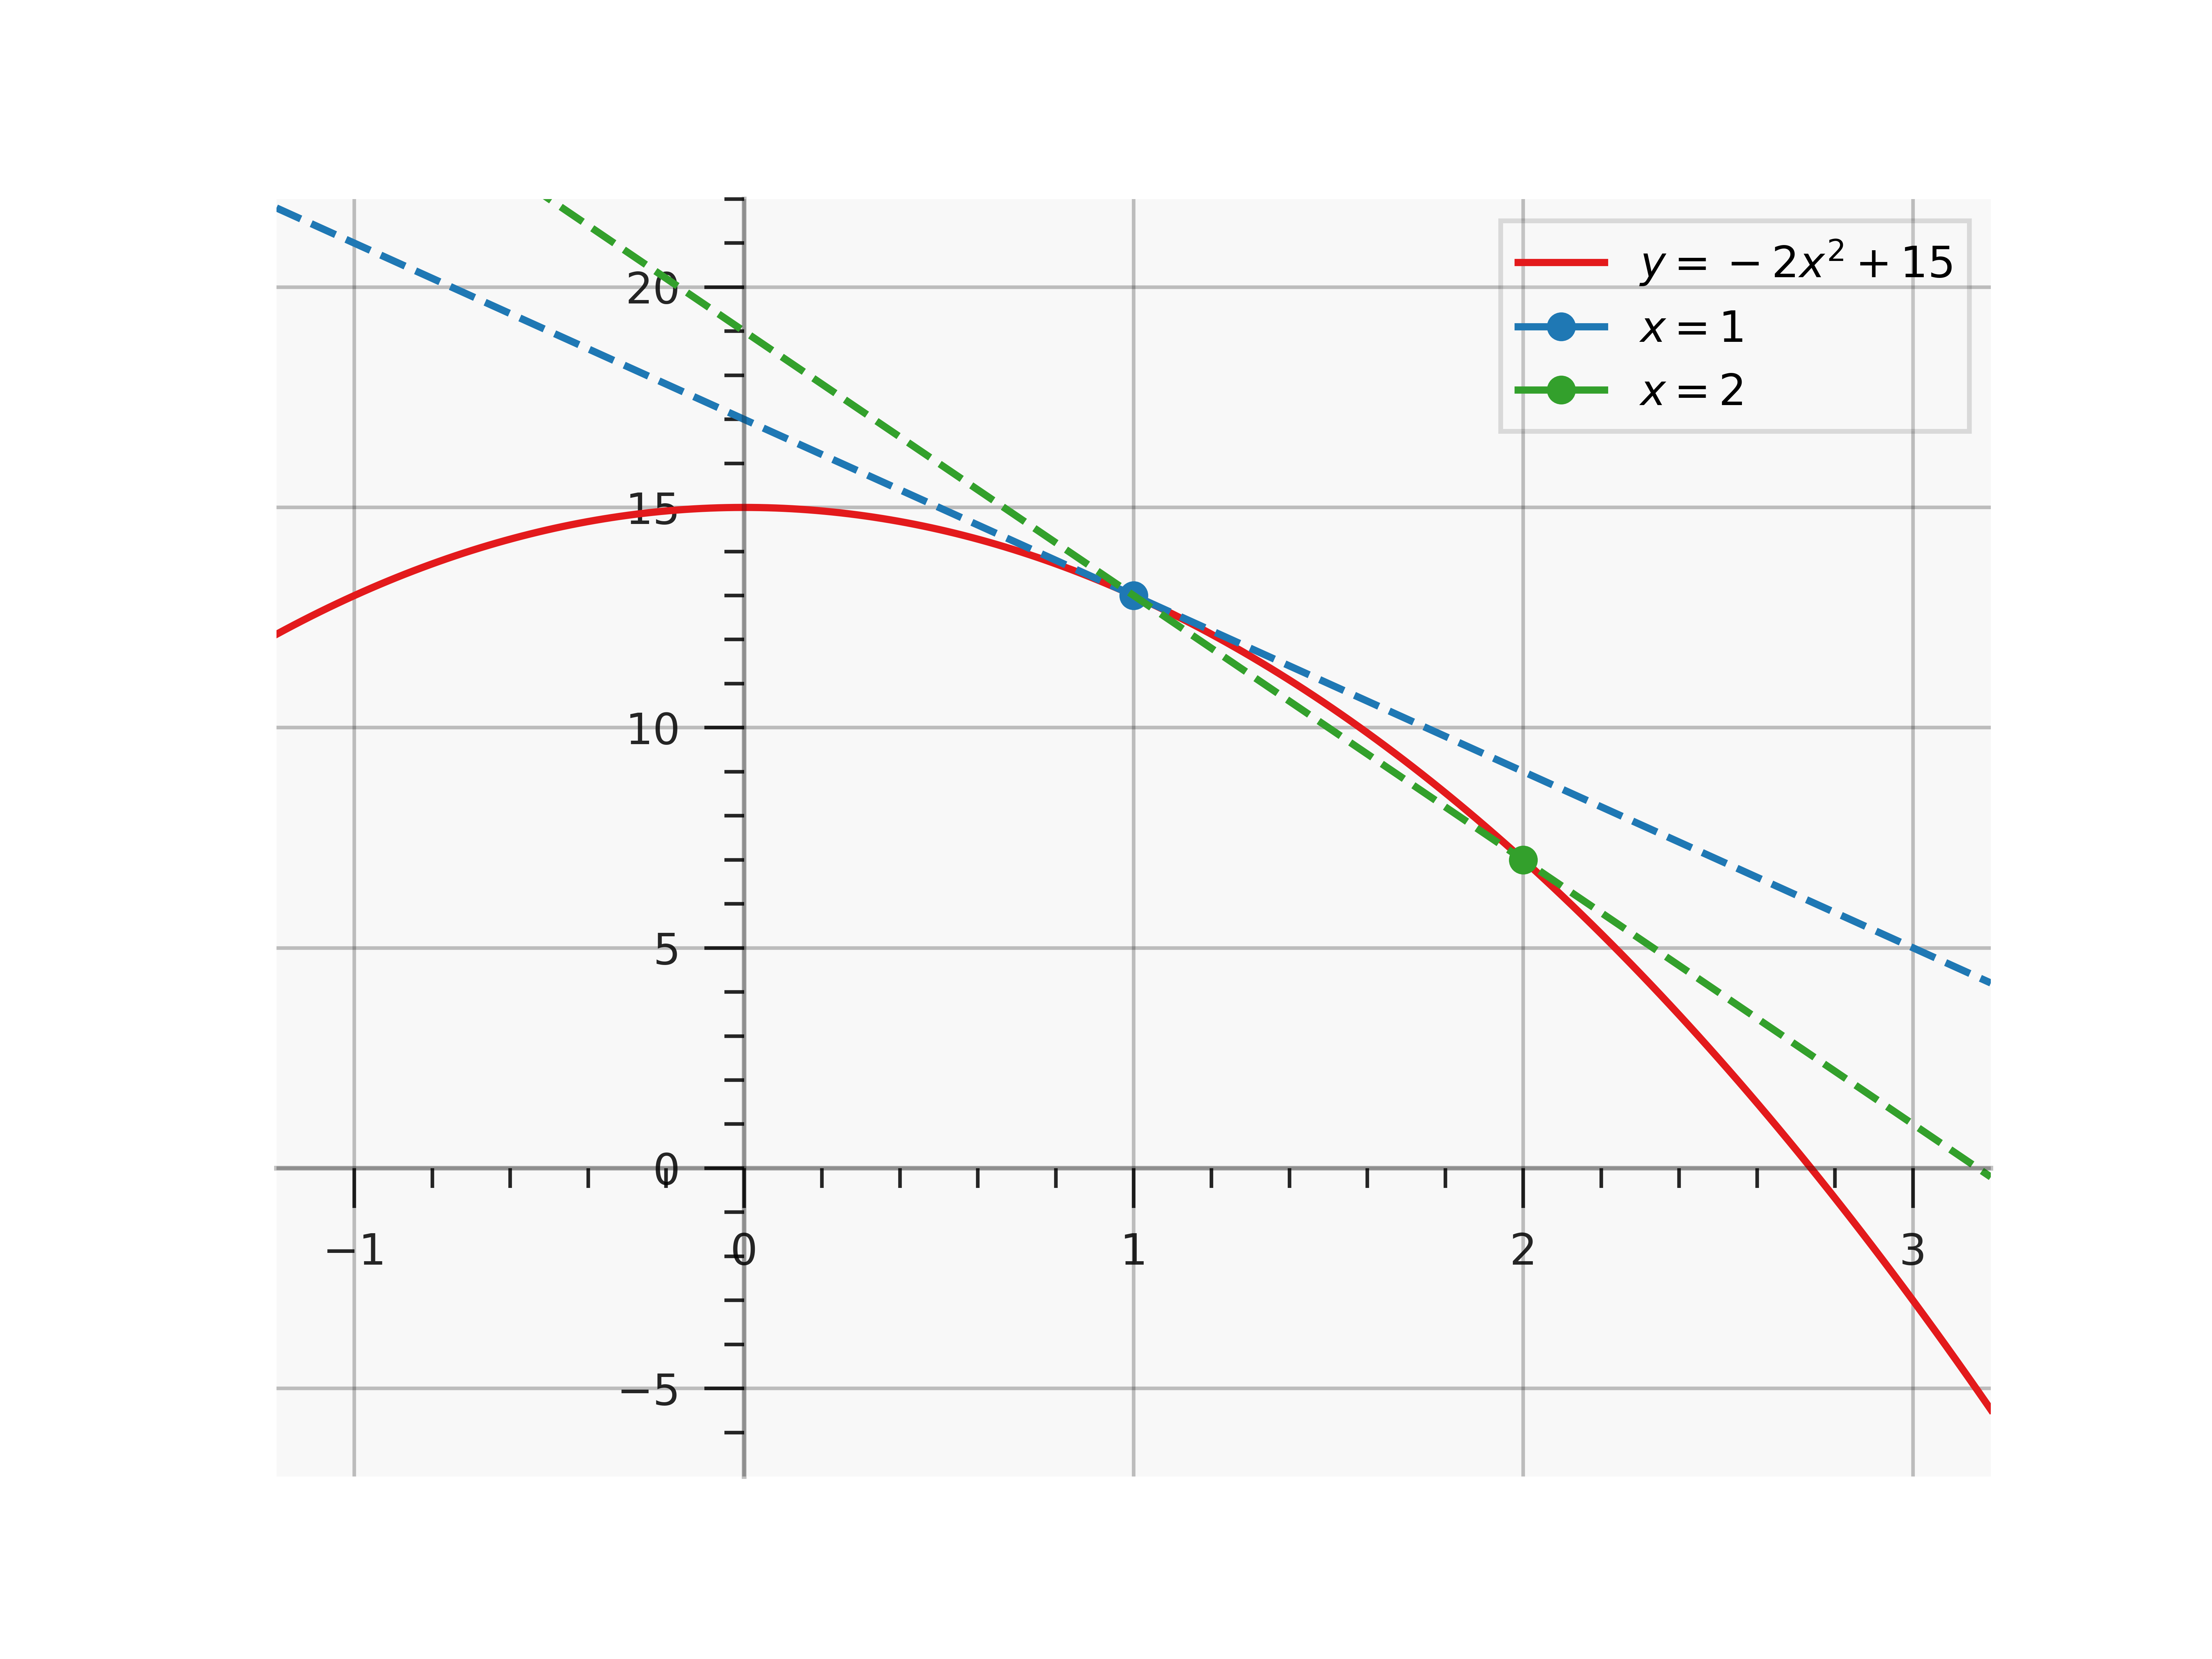
\includegraphics[width=12.5cm, keepaspectratio]{tangent_lines_2.png}
    \caption{Approximating Tangent Lines}
    \label{fig:fig2}
\end{figure}

We can see that the tangent line in blue is somewhat similar to the secant line in green.
We would expect their slopes to be similar as well.
The slope of the secant line, $m_{PQ}$, and by extension an approximation of the slope of the tangent line, is:

\begin{equation*}
    m_{PQ} = \frac{f(2)-f(1)}{2-1} = \frac{7-13}{1} = -6
\end{equation*}

That is an estimate of the slope of the tangent line, but not the best estimate.
We can improve it by using values of $x$ for $Q$ that are closer to $x=1$.
Calculuting the slope of the secant line connecting $P$ and $Q$ would be more accurate than what we calculated above.
That is, the closer point $Q$ is to $P$, the closer the secant line connecting them is to the tangent line.
Thus, the values of the slopes of the two lines would get closer to each other.

We can use that to see that the slopes of the lines would be the same if $Q$ used $x=1$.
However, that would make it the same as point $P$ so it defeats the purpose of getting two points on the tangent line to calculate its slope; the $x_2-x_1$ part of the slope formula would be $1-1=0$, and we cannot divide by 0 anyways.
Instead, we will use values of $x$ that are getting closer and closer to $x=1$ to get better and better estimates of the slope of the tangent line.
To do this, we can make a general slope formula for the secant line for any value of $x$.
For $Q=(x, f(x))$, that would be:

\begin{equation}
    m_{PQ} = \frac{f(x)-f(1)}{x-1} = \frac{-2x^2 + 15 - 13}{x-1} = \frac{-2x^2+2}{x-1}
\end{equation}

Note that so far we have only consider values of $x$ for $Q$ that are greater than $x=1$.
That is, we have only looked at when $Q$ is to the right of $P$.
We can, and should, look at values to the left of $Q$ as well.
While in this case, the same thing is happening for $Q$ to the left or right of $P$, this is not always the case.
Below is a table of values of $x$ versus $m_{PQ}$ using the above formula.

\begin{table}[h]
    \renewcommand{\arraystretch}{1.5}
    \centering
    \begin{tabular}{>{\centering\arraybackslash}m{1.5cm}|>{\centering\arraybackslash}m{1.5cm}|>{\centering\arraybackslash}m{1.5cm}|>{\centering\arraybackslash}m{1.5cm}}
        $x$      & $m_{PQ}$  & $x$      & $m_{PQ}$  \\ \hline
        $2$      & $-6$      & $0$      & $-2$      \\
        $1.5$    & $-5$      & $0.5$    & $-3$      \\
        $1.1$    & $-4.2$    & $0.9$    & $-3.8$    \\
        $1.01$   & $-4.02$   & $0.99$   & $-3.98$   \\
        $1.001$  & $-4.002$  & $0.999$  & $-3.998$  \\
        $1.0001$ & $-4.0002$ & $0.9999$ & $-3.9998$
    \end{tabular}
\end{table}

We can see that $m_{PQ}$ seemingly approaches $-4$ as $Q$ uses values of $x$ closer to 1.
This is the case when we approach $x=1$ from both the right and left, using values smaller and larger than it.
From this, we can estimate the slope of the tangent line to be $-4$.
It is also the case $-4$ is the actual slope of the tangent line, which we may prove with some more knowledge of calculus.

The equation of a line which passes through $(a, f(a))$ is given by the following, which can be gotten from the point-slope form of a linear equation.

\begin{equation}
    y = f(a) + m(x-a) \label{eq:2}
\end{equation}

Then, the equation of the line tangent to $f(x)=-2x^2+15$ at $x=1$ and the solution to Problem~\eqref{eq:1} is:

\begin{equation}
    y = 13 - 4(x-1) = -4x + 17
\end{equation}

The first to note with our problem is that we we looked at both sides of $x=1$ to determine the trend.
It is important to not assume that what happens on one side will happen on the other.
From how the graph looked in our example, it was safe to assume that such an assumption would be true.
Usually we would not have a graph to determine this, and it would be difficult to get one.

Also, when using values of $x$ that are 'close' to our target value, we went quite close.
This makes it to assume that the actual value will fit the trend that we have observed.
It was almost lucky that the values of the slope converged rather quickly with only a few computations.
For most values, they will be quite a bit 'messier' and more computations will be needed.
In general, at least 4 values of $x$ should be used on each side to get a good estimate; values should be closer and closer to the target $x$ value until the differences between successive points becomes very small.

Finally, we could not plug $x=1$ into our slope formula as that would make us divide by 0, which we cannot do.
However, we were still able to plug in values close to it and infer a trend from that to find the slope at $x=1$.
This idea is rather important and will be covered in later sections.

What we have done is found a the equation of the line tangent to $f(x)$ at a point $x=a$.
We know one point on the line is $P=(a, f(a))$.
Using values of another point $Q=(x,f(x))$, the slope of the secant line between those two points is given by the following formula.

\begin{equation}
    m_{PQ} = \frac{f(x)-f(x)}{x-a}
\end{equation}

With values of $x$ closer and closer to $a$ (on both sides of point $P$), we used the general trend to estimate the slope of the tanget as $m$.
The equation of the tangent line is then given by Equation \eqref{eq:2}.

\section{Rates of Change}
As stated before, this is one of the most important concepts in Calculus I.
We will consider some function $f(x)$, representing some quantity which varies as $x$ varies; $f(x)$ represent the volume of tank changing with time, or the distance travelled by a car changing with time.
$x$ does not have to represent time but it may be easier to visualise examples where it does.
We want to find out how fast $f(x)$ changes at some point $x=a$.
This may be referred to as the \textbf{instantaneous rate of change} or the rate of change of $f(x)$ at $x=a$.

As with our tangent problem, we are currently only able to estimate it.
We may not be able to find the instantaneous rate of change, but we can find the average rate of change.
This is done by using another point, say $x$; the average rate of change between these two points is:

\begin{align}
    A.R.C. & = \frac{\text{change in } f(x)}{\text{change in } x} \\
           & = \frac{f(x)-f(a)}{x-a}
\end{align}

The $A.R.C.$ becomes a better and better estimate for the instantaneous rate of change as we use values of $x$ closer to $x=a$.
Once again, we need to use values on both sides of $x=a$ to get the trend from which we can estimate the instantaneous rate of change.
Below is an example of a rate of change problem.

\begin{problem}
Suppose that volume of air in a balloon after $t$ hours is given by,

\begin{equation}
    V(t) = t^3 - 6t^2 + 35 \label{eq:3}
\end{equation}

Estimate the instantaneous rate of change of the volume after 5 hours.
\end{problem}

We want to find the instantaneous rate of change of $V(t)$ at $t=5$.
First, we shall get a formula for the average rate of change between some point and some other value of $t$.

\begin{equation}
    A.R.C. = \frac{V(t)-V(5)}{t-5} = \frac{t^3-6t^2+35-10}{t-5} = \frac{t^3-6t^2+25}{t-5}
\end{equation}

Now, we can estimate the instantaneous rate of change by using values of $t$ close to 5 and computing the $A.R.C.$
The following table does just that.

\begin{table}[h]
    \renewcommand{\arraystretch}{1.5}
    \centering
    \begin{tabular}{>{\centering\arraybackslash}m{1.5cm}|>{\centering\arraybackslash}m{2.5cm}|>{\centering\arraybackslash}m{1.5cm}|>{\centering\arraybackslash}m{2.5cm}}
        $t$      & $A.R.C.$      & $t$      & $A.R.C.$      \\ \hline
        $6$      & $25$          & $4$      & $7$           \\
        $5.5$    & $19.75$       & $4.5$    & $10.75$       \\
        $5.1$    & $15.91$       & $4.9$    & $14.11$       \\
        $5.01$   & $15.0901$     & $4.99$   & $14.9101$     \\
        $5.001$  & $15.009001$   & $4.999$  & $14.991001$   \\
        $5.0001$ & $15.00090001$ & $4.9999$ & $14.99910001$
    \end{tabular}
\end{table}

We can see that the $A.R.C.$ is appraoching 15 from both sides of $x=5$.
Hence, the instantaneous rate of change at $x=5$ can be estimated to be 15.
That is the solution to Problem~\eqref{eq:3}.

To assign some meaning to our solution, we shall suppose that the units of volume are \si{cm^3}.
That means that units of the rates of change are \si[per-mode=symbol]{cm^3/hr}.
At $t=5$, the volume of the balloon is changing at a rate of 15\si[per-mode=symbol]{cm^3/hr}.
That means that 5 hours after the starting time, if the rate of change was constant, the balloon would gain 15\si{cm^3} of air an hour later.

Now, that does not necessarily that were will be 15\si{cm^3} more air in the balloon at $t=6$ versus $t=5$ because the rate of change is changing with time.
What we can say is that the volume is increasing at $t=5$ and we can compare it to other values of $t$.
For instance, the instantaneous rate of change at $t=4$ is 0\si[per-mode=symbol]{cm^3/hr} and at $t=3$ it is -9\si[per-mode=symbol]{cm^3/hr}.
Both of these can be easily verified in the same way as was done for $t=5$ above.

At $t=4$, the rate of change is 0\si[per-mode=symbol]{cm^3/hr}, meaning that the volume is not changing at that point in time; all this says is that the volume is constant at that specific point and not whether it will change in the future.
The rate of change being negative at $t=3$ means that the volume of air in the balloon is decreasing at that point.
We may state, ignoring whether the volume is increasing or decreasing (hence ignoring the negative sign in -9\si[per-mode=symbol]{cm^3/hr}), that the volume of air in the balloon is changing faster at $t=5$ than $t=3$ as 15 is greater than 9.

Rates of change will be discussed a lot when considering derivatives.
Before that, we may wish to consider the velocity problem; this is really just a special case of the rate of change problem.
Say that the position of an object is described by the function $f(t)$, giving the position of the object at time $t$.
Then, the instantaneous velocity may be computed by recognising the fact that velocity is the rate of change of position.
The average velocity between time $t$ and $a$ is given by the following.

\begin{equation}
    A.V. = \frac{\text{change in position}}{\text{change in time}} = \frac{f(t)-f(a)}{t-a}
\end{equation}

By evaluating the average rate of change with values of $t$ getting closer and closer to $t=a$, we get better and better estimates of the instantaneous velocity.

\section{Change of Notation}
The purpose of this is to introduce some key concepts that relate to the concept of limits.
Before that, we may change the notation used by a bit to better relate the tangent and rate of change problems to limits.
First, note that whether we were finding the slope of a tangent line or the rate of change of some quantity with respect to time, we used the exact same formula.
That is the following.

\begin{equation}
    \frac{f(x)-f(a)}{x-a} \label{eq:4}
\end{equation}

That would suggest that all of the problems covered are really the same thing.
The only difference is what we are representing with our solutions.
To prepare for the discussion of limits officially, one simple change of notation will be useful.

In our problems, we have considered $x=a$ and have defined a new point in reference to it.
If we want to move some distance $h$ from $x=a$, then we would have $x=a+h$ as our new point.
To get points to the right of $x=a$, we use $h>0$; we use $h<0$ for points to the left of $x=a$.
With this way of writing our second value, we can change Equation~\eqref{eq:4} to get the following.

\begin{equation}
    \frac{f(x)-f(a)}{x-a} = \frac{f(a+h)-f(a)}{a+h-a} = \frac{f(a+h)-f(a)}{h}
\end{equation}

Now, this is the formula for specific values of $x$, $x=a$.
Usually, we don't care about that and just want a general formula.
That would be the following, replacing $a$ with $x$.

\begin{equation}
    \frac{f(x+h)-f(x)}{h} \label{eq:5}
\end{equation}

While this may seem overly complicated, it will make it easier to deal with problems if we use this form.
We shall see this with the discussion of limits and derivatives.

\end{document}